\documentclass[11pt,a4paper]{article}

\usepackage[polish]{babel}
\usepackage[utf8]{inputenc}
\usepackage{polski}
\usepackage[T1]{fontenc}
\usepackage{indentfirst}
\usepackage{wrapfig}    % for wrapping figures, tables

\frenchspacing

%\usepackage{amsmath}
\usepackage{physics}
%\usepackage{bm}
\usepackage{gensymb}
%\usepackage{hepnames}
\usepackage{epsfig}
\usepackage{graphics}
\usepackage[shortlabels]{enumitem}
%\usepackage{xspace}
%\xspaceaddexceptions{[]\{\}}

%
%
%fixpagesize
\pagestyle{empty}
\addtolength{\textwidth}{6cm}
\addtolength{\textheight}{4cm}
\addtolength{\evensidemargin}{-3cm}
\addtolength{\oddsidemargin}{-3cm}
\addtolength{\topmargin}{-2cm}
\parindent=0cm

%
%
%small distance in list/item/enum for enumitem package
\setlist[itemize,enumerate]{topsep=0em}
\setlist{noitemsep}


% definition of inexact differential symbol:
\newcommand{\dbar} {\ensuremath{\,\mathchar'26\mkern-12mu d}}

%print zadanie #
\newcounter{zadanie}\newcommand{\zadanie}[1][]{\addtocounter{zadanie}{1} ~\\  {\bf \emph{Zadanie \arabic{zadanie} #1 }} \\}
\newcounter{zaddom}\newcommand{\zaddom}[1][]{\addtocounter{zaddom}{1} ~\\  {\bf \emph{Zadanie domowe \arabic{zaddom} #1 }} \\}
%\renewcommand{\zadanie}[1][]{\pagebreak  ~\\  {\bf \emph{Zadanie }} \\} \addtolength{\topmargin}{-2cm}


%
%%%%%%%%%%%%%%%%%%%%%%%%%%%%%%%%%%%%%%%%%%%%%%%%%%%%%%
% Changes figure placing algorithm
\renewcommand{\topfraction}{1}       % maximal fraction of a page allowed for figures
\renewcommand{\textfraction}{0.15}   % minimal number of text for figure-text shared pages
\renewcommand{\floatpagefraction}{0.95} % if two above does not help, this could do the job
                                        % must be: floatpagefraction < topfraction !!!!
%
\renewcommand{\textfraction}{0} % minimum fraction of page, which must be
                                % devoted to text
\renewcommand{\topfraction}{1}  % maximum fraction at top, which can be
                                % occupied whit floats
\setcounter{totalnumber}{400}   % increase the number of floats for one page
\setcounter{topnumber}{200}     % at all/top/bottom.
\setcounter{bottomnumber}{200}  %


\begin{document}           % End of preamble and beginning of text.
\begin{centering}
\bf{\Large{Termodynamika z elementami fizyki statystycznej}}\\
Tydzień 12 (25 maja 2023)\\[5mm]
Rozkład Boltzmanna, entropia \\
\end{centering} 
\vspace{5mm}

\begin{wrapfigure}[3]{r}{0.2\linewidth}\vspace{-5mm}
\resizebox{\linewidth}{!}{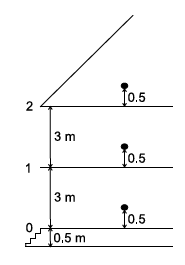
\includegraphics{szewc.png}}
\end{wrapfigure}
\zadanie
Szewc ma na rynku wąski domek o 3 kondygnacjach. W ciągu doby średnio:
\begin{itemize}
\item 4 h 35 min. spędza w kuchni na 2 piętrze,
\item 7 h 25 min. śpi w sypialni na 1 piętrze,
\item 12 h pracuje w warsztacie na parterze.
\end{itemize}
(a) Jakie jest prawdopodobieństwo znalezienia szewca na poziomie 0, 1 oraz 2?\\
(b) Jaka jest średnia wysokość środka masy szewca w ciągu doby (patrz rysunek)?\\
(c) Jaka jest średnia energia potencjalna szewca ($m=50$ kg)?\\
(d) Czy opisany układ mógłby być rozkładem termicznym? \\

{\em Rozwiązanie:} Odpowiednie prawdopodobieństwa liczymy jako ułamek czasu jaki szewc spędza na każdej kondygnacji
\begin{equation}
	p_2 = \frac{275\,{\rm min}}{1440\,{\rm min}} = \frac{55}{288}, \quad p_1 = \frac{445\,{\rm min}}{1440\,{\rm min}} = \frac{89}{288}, \qquad  p_0 = \frac{720\,{\rm min}}{1440\,{\rm min}} = \frac{1}{2}.
\end{equation}
Średnia wysokość środka masy szewca wynosi
\begin{equation}
	\langle h \rangle = p_0 h_0 + p_1 h_1 + p_2 h_2 = 3.07\,{\rm m},
\end{equation}
gdzie, zgodnie z rysunkiem, $h_0 = 1\,{\rm m}$, $h_1 = 4\,{\rm m}$, $h_2 = 7\,{\rm m}$. Średnia energia potencjalna szewca wynosi $\langle E_p \rangle = m g \langle h \rangle = 1506\,{\rm J}$.

By sprawdzić, czy rozkład częstości występowania szewca na danym piętrze ma szanse być rozkładem termicznym, względne prawdopodobieństwa powinny spełniać rozkład Boltzmanna, to znaczy
\begin{equation}
	\frac{p_i}{p_j} = \exp\left( - (E_i - E_j)/ (k T)\right),
\end{equation}
gdzie $E_i$ jest energią potencjalną szewca na $i$-tym poziomie. Wyznaczając z tego równania $T$ dostajemy
\begin{equation}
	kT = - \frac{E_i - E_j}{\log p_i / p_j} = - mg \frac{h_i - h_j}{\log p_i/p_j}.
\end{equation}
Rozważając różne możliwości otrzymujemy
\begin{equation}
	\frac{h_1- h_0}{\log p_1/p_0} \approx - 6.235, \quad \frac{h_2- h_1}{\log p_2/p_1} \approx -6.233, \quad \frac{h_2- h_0}{\log p_2/p_0} \approx -6.234.
\end{equation}
Widzimy więc, że dany rozkład nie jest ściśle rozkładem termicznym, ale jest nim w bardzo dobrym przybliżeniu i możemy szewcowi ''przypisać'' przybliżoną temperature
\begin{equation}
	T = 6.234\, \frac{m g}{k} = 2.21 \times 10^{26}\,{\rm K}.
\end{equation}
Temperatura jest ogromna, ponieważ szewc znajduję się w stanach o bardzo różnej, z punktu widzenia mikroskopowego, energii.

\newpage


\zadanie
Pewna cząsteczka ma, poza stanem podstawowym o zerowej energii, dwa stany wzbudzone o energiach $\varepsilon$ i $2\,\varepsilon$.
Obserwując 1 mol takich (rozróżnialnych) cząsteczek stwierdzono, że w wymienionych stanach przebywa odpowiednio 4/7, 2/7 i 1/7 cząsteczek.
\begin{enumerate}[a)]
\item Znajdź entropię układu licząc mikrostany. 
\item Znajdź entropię korzystając ze wzoru Gibbsa.
\end{enumerate}
Stała Boltzmanna wynosi $k = 1.38\cdot 10^{-23}\,$J/K, 
liczba Avogadra $N_A=6.02\cdot 10^{23}$\, mol$^{-1}$. \\
%$R=8.31$\,J/mol/K. 
Jaki jest zakres stosowalności wzorów z pkt. a) i b)?

{\em Rozwiązanie:}
\begin{enumerate}[a)]
\item cząstka ma $3$ stany oraz jest $N = 1\,{\rm mol} \cdot N_A$ cząstek. Ilość konfiguracji wynosi więc $\Omega = 3^{N}$, a entropia
\begin{equation}
	S = k \log \Omega = k N \log 3 \approx 9.13\,{\rm J/K} \label{A}
\end{equation}
Przy liczeniu liczby konfiguracji możemy też uwzględnić, że różne stany są obsadzone z różnym prawdopobieństwem. Wtedy liczba konfiguracji
\begin{equation}
	\Omega = \binom{N}{\frac{4}{7}N} \binom{\frac{3}{7}N}{\frac{2}{7}N} = \frac{N!}{(\frac{4}{7}N)! (\frac{2}{7}N)! (\frac{1}{7}N)!}.
\end{equation}
Korzystając z przybliżenia Stirlinga dla logarytmu silni,
\begin{equation}
	\log n! = n \log n + \mathcal{O}(n),
\end{equation}
dostajemy
\begin{align}
	S &= k \left(N \log N - 4/7 N \log 4/7 N - 2/7 N \log 2/7 N - 1/7 N \log 1/7 N\right) \nonumber \\
	&= - k N \left(4/7 \log 4/7 + 2/7 \log 2/7 + 1/7 \log 1/7)\right), \label{B}
\end{align}
czyli tak jak w drugiej części, ponieważ

\item zgodnie z wzorem Gibbsa, entropia wynosi
\begin{equation}
	S = - k N (p_0 \log p_0 + p_1 \log p_1 + p_2 \log p_2) \approx 7.94\,{\rm J/K}
\end{equation}
\end{enumerate}
Wzór~\eqref{A} jest szczególnym przykładem wzoru Gibbsa w sytuacji gdy każdy ze stanów jest realizowany z takim stanym prawdopodobieństwem .Wzór~\eqref{B} otrzymaliśmy licząc mikroskopową liczbę stanów zgodnych z makroskopową obserwacją prawdopodobieństwa z jakim cząstki znajdują się w odpowiednich stanach i przy założeniu, bardzo dużej liczby cząstek, tak by tylko wiodący wyraz w rozwinięciu $\log n!$ był istotny.

\newpage


\zadanie
Pewna cząsteczka ma, poza stanem podstawowym o zerowej energii, dwa stany wzbudzone o energiach $\varepsilon$ i $2\,\varepsilon$.
Obserwując zespół wielu takich cząsteczek pozostających w równowadze z 
termostatem stwierdzono, że średnio 4/7 z nich jest w stanie podstawowym.
\begin{enumerate}[a)]
\item Jaka jest temperatura układu? 
      Jaki ułamek cząsteczek jest w stanie najwyższego wzbudzenia?
\item W powyższym układzie znalazła się jedna cząsteczka innego typu, 
      mająca dwa różne stany wzbudzone, ale oba o tej samej energii $2\,\varepsilon$. 
      Jakie jest prawdopodobieństwo znalezienia jej w stanie podstawowym?
\end{enumerate}

{\em Rozwiązanie:}
\begin{enumerate}[a)]
\item Z treści zadania wiemy, że $p_0 = 4/7$ oraz $E_0 = 0$. Ze związku $p_0 = e^{-\beta E_0}/Z$ wynika więc $Z=7/4$. Z drugiej strony funkcja rozkładu jest dana przez
\begin{equation}
	Z = 1 + e^{-\beta \epsilon} + e^{-2 \beta \epsilon} = 1 + x + x^2,
\end{equation}  
z $x = exp(-\beta \epsilon) > 0$. Rozwiązując, znajdujemy $x = 1/2$, z czego wynika, że $T = \epsilon / (k \log 2)$. Prawdopodobieństwo, że cząstka jest w stanie o najwyższej energii wynosi
\begin{equation}
	p_3 = \frac{e^{-2 \beta \epsilon}}{Z} = \frac{4}{7} \left( \frac{1}{2}\right)^2 = \frac{1}{7}.
\end{equation}
\item Funkcja rozkładu nowej cząstki, zakładając, że układ jest w tej samej temperaturze wynosi
\begin{equation}
	Z_2 = 1 + 2 e^{-2\beta \epsilon} = 1 + 2 \cdot \frac{1}{4} = \frac{3}{2}.
\end{equation}
Stąd, prawdopobieństwo, że nowa cząstka jest w stanie podstawowym wynosi $2/3$. 
\end{enumerate}

\newpage

\zadanie
{\em Dwupoziomowy (kwantowy) model paramagnetyzmu}\\
W jednorodnym zewnętrznym polu magnetycznym o indukcji $\vec{B}$
znajduje się atom o spinie $\frac{1}{2}$ i momencie magnetycznym $\vec{\mu}_0$.
Moment magnetyczny atomu może być ustawiony albo równolegle albo antyrównolegle do
zewnętrznego pola magnetycznego, a energia oddziaływania z tym polem wynosi
$\displaystyle E = - \vec{\mu}_0 \cdot \vec{B}$.
Układ znajduje się w równowadze z termostatem o temperaturze $T$.
\begin{enumerate}[a)]
\item Obliczyć średni moment magnetyczny atomu,
\item Przedyskutować wynik w granicy $\mu_0 B \gg k T$ (tj. silne pole, niska temperatura) oraz $\mu_0 B \ll k T$ (tj. słabe pole, wysoka temperatura),
\item Pamiętając, że: podatnością magnetyczną $\chi$ nazywa się współczynnik proporcjonalności między namagnesowaniem materiału $\vec{M}$ a polem $\vec{B}$,
zaś namagnesowanie $\vec{M}$ jest momentem magnetycznym na jednostkę 
objętości materiału, wykazać, że w granicy słabych pól magnetycznych dla naszego modelowego paramagnetyka spełnione jest prawo Curie:
$\displaystyle \chi = \frac{C}{T}$,
gdzie $C$ jest pewną stałą, nazywaną stałą Curie.
\end{enumerate}

{\em Rozwiązanie:}

Przyjmijmy, że zewnętrzne pole magnetyczne jest skierowane w górę. Prawdopodobieństwa, że spin jest skierowany równolegle lub antyrównolegle do pola magnetycznego wynoszą
\begin{equation}
	p_{\uparrow} = \frac{e^{- \beta \mu_0 B}}{Z}, \qquad p_{\downarrow} = \frac{e^{ \beta \mu_0 B}}{Z},
\end{equation}
z funkcją rozkładu daną przez
\begin{equation}
	Z = e^{- \beta \mu_0 B} + e^{ \beta \mu_0 B} = 2 \cosh \beta \mu_0 B.
\end{equation}
\begin{enumerate}[a)]
	\item Średni moment magnetyczny $\langle \mu \rangle = +\mu_0 p_{\uparrow} - \mu_0 p_{\downarrow} = \mu_0 \tanh \beta \mu_0 B$. 
	\item Przypadki graniczne: 
	\begin{itemize}
	\item W granicy $\mu_0 B \gg k T$ mamy $\beta \mu_0 B \gg 1$. Funkcja $\tanh(x)$ dla dużych argumentów dąży do $1$, więc $\langle \mu \rangle \rightarrow \mu_0$.
	\item Dla słabych pól i wysokich temperatur $\beta \mu_0 B \ll 1$. Funkcja $\tanh(x) = x + \mathcal{O}(x^3)$ dla małych argumentów więc $\langle \mu \rangle = \mu_0^2 B / (k_B T)$.
	\end{itemize}
	\item Oznaczmy przez $n$ liczbę atomów na jednostkę objętości. Wtedy namagnesowanie $M$ wynosi $M = n \langle \mu \rangle$. Dla słabych pól, korzystając w wyniku z poprzedniego punktu dostajemy
	\begin{equation}
		M = \frac{n \mu_0^2}{k_B T} B = \chi B, \qquad \chi = \frac{n \mu_0^2}{k_B} \frac{1}{T}.
	\end{equation}
	Stała Curie wynosi więc $C = n \mu_0^2/k_B$.
	
\end{enumerate}

\newpage

\zadanie
Udowodnij, że dla cząstki będącej w równowadze z termostatem o temperaturze $T$ i 
podlegającej rozkładowi Boltzmanna spełnione są tożsamości:
\[ \langle E\rangle = - \frac{1}{Z} \cdot \frac{\partial Z}{\partial \beta}, ~~~~
\langle E^2\rangle = \frac{1}{Z} \cdot \frac{\partial^2 Z}{\partial \beta^2}, \]
gdzie: $E$ - energia cząstki, $Z$ - suma statystyczna, $\beta = \frac{1}{k T}$.
Rozważ przypadki dyskretnych i ciągłych stanów energetycznych.

{\em Rozwiązanie:}

W przypadku dyskretnym, funkcja rozkładu dana jest przez
\begin{equation}
	Z = \sum_i e^{-\beta E_i},
\end{equation}
gdzie $E_i$ jest energią cząstki w stanie $i$, suma jest po wszystkich możliwych stanach cząstki. Średnia energia wynosi
\begin{equation}
	\langle E \rangle = \sum_i E_i p_i,
\end{equation}
gdzie $p_i = e^{-\beta E_i}/Z$. Możemy teraz wykonać parę przekształceń
\begin{equation}
	\langle E \rangle = \frac{1}{Z}\sum_i E_i e^{-\beta E_i} = \frac{1}{Z} \sum_i (-\partial_{\beta}) e^{-\beta E_i} = -\frac{1}{Z} \partial_{\beta} \left(\sum_i e^{-\beta E_i}\right) = - \frac{1}{Z} \partial_{\beta} Z = - \partial_{\beta} \log Z.
\end{equation}

Drugą równość rozważmy dla przykładu ciągłego. Niech $E(x)$ i $p(x)$ będą energią cząstki w stanie $x$ oraz prawdopodobieństwem, że cząstka jest w tym stanie. Mamy
\begin{equation}
	\langle E^2 \rangle = \int {\rm d}x\, E^2(x) p(x) = \frac{1}{Z} \int {\rm d}x\, E^2(x) e^{-\beta E(x)} = \frac{1}{Z} \int {\rm d}x\, \partial_{\beta}^2\, e^{-\beta E(x)} = \frac{1}{Z}\partial_{\beta}^2  \int {\rm d}x\, e^{-\beta E(x)} = \frac{1}{Z}\partial_{\beta}^2 Z,
\end{equation}
z funkcją rozkładu daną przez
\begin{equation}
	Z = \int {\rm d}x\, e^{-\beta E(x)}.
\end{equation}

\newpage 
\zadanie
Energie stanów rotacyjnych cząsteczek dwuatomowych dane są wzorem: $E_j = j(j+1)\varepsilon$,
gdzie $j=0,1,2,...$, a $\varepsilon$ jest stałą. 
Dla każdej warości $j$  występuje $2j+1$ różnych stanów o tej samej energii $E_j$. 
Oblicz średnią energię takiej cząsteczki w warunkach równowagi termodynamicznej 
z termostatem o temperaturze $T$ przy założeniu, że $kT \gg \varepsilon$, gdzie $k$ - stała Boltzmanna.

{\em Rozwiązanie:} 

Zacznijmy od zapisania funkcji rozkładu. Możemy zapisać ją jako sumę po wszystkich stanach, lub biorąc pod uwagę degenerację (różne stany mają tą samą energie) możemy napisać
\begin{equation}
	Z = \sum_{j=0}^{\infty} (2j+1) e^{-\beta E_j} = \sum_{j=0}^{\infty} (2j+1) e^{-\beta j(j+1) \epsilon}.
\end{equation}
By obliczyć $Z$ skorzystamy z założenia, że $kT \gg \varepsilon$ czyli $\beta \varepsilon \ll 1$. W tej sytuacji możemy przybliżyć sumę za pomocą całki korzystając ze wzoru Eulera-Maclaurina
\begin{equation}
	\sum_{n=a}^b f(n) = \int_{a}^b {\rm d}n f(n) + \frac{f(b) + f(a)}{2} + \frac{1}{6} \frac{f'(b) - f'(a)}{2} + \dots
\end{equation}
gdzie $\dots$ oznaczają wyrazy z coraz wyższymi pochodnymi. W rozważanym przypadku mamy $f(x) = (2x+1) \exp(-\beta \epsilon x(x+1))$ i dostajemy
\begin{equation}
	\int_0^{\infty} {\rm d}x (2x +1) e^{- \beta \epsilon (x^2+x)} = - \frac{1}{\beta \epsilon} \int_{0}^{\infty} \partial_x e^{-\beta \epsilon (x^2+x)} = \frac{1}{\beta \epsilon}.
\end{equation}
oraz
\begin{equation}
	f(0) = 1, \qquad f(\infty) = 0, \qquad f'(0) = 2 - \beta \epsilon, \qquad f'(\infty) = 0.
\end{equation}
Czyli
\begin{equation}
	Z = \frac{1}{\beta \epsilon} + \frac{1}{2} - \frac{1}{12}(2 - \beta \epsilon) + \dots \approx \frac{1}{\beta \epsilon},
\end{equation}
ponieważ $\beta \epsilon$ jest małą liczbą więc jej odwrotność jest dużo większe od $1$. Średnią energie możemy terez policzyć ze związku wyprowadzonego w poprzednim zadaniu. Dostajemy
\begin{equation}
	\langle E \rangle = - \frac{1}{Z} \partial_{\beta} Z = \beta \epsilon \frac{1}{\beta^2\epsilon} = k_B T.
\end{equation}

\end{document}
